\documentclass[a4paper,12pt]{article}

\usepackage{amsmath,amssymb,amsthm,tikz}
\usetikzlibrary{calc,arrows.meta}
\usepackage[margin=20mm]{geometry}
\usepackage{fancyvrb}
\usepackage{enumerate}
\usepackage{hyperref}

\setlength{\parindent}{0pt}
\setlength{\columnsep}{1cm}

\newcommand{\indsize}{\scriptsize}
\newcommand{\colind}[2]{\displaystyle\smash{\mathop{#1}^{\raisebox{.5\normalbaselineskip}{\indsize #2}}}}
\newcommand{\rowind}[1]{\mbox{\indsize #1}}

\begin{document}
\thispagestyle{empty}

\twocolumn

\begin{center}
{\Large Final and Solution. 2020-12-17.}\\
{\em 120 minutes.} 
\end{center}


% 
\vspace{10pt}
{\bf Question 1 (Using STL).} 

%% One could ask to run a strange algorithm like this:
%% https://www.geeksforgeeks.org/search-in-row-wise-and-column-wise-sorted-matrix/
%% https://en.cppreference.com/w/cpp/types/size_t



There is a datatype {\tt Student} to store student data. 
Students are not allowed to change their
birthdates and their names while studying ({\tt birth} shows 
how many days separate January 1, 1970 and their birthday).

\vspace{5pt}
You want to store these students in an STL 
data structure {\tt unordered\textunderscore{}set} 
that would allow to iterate over them (and also insert new students
or remove them once they graduate). 

This STL class requires that you implement a hashing function and
an equals operator.
In this task you will write your own hashing function
(and also evaluate, if other hash functions are good for this task).

\vspace{5pt}
{\bf (A)} Write your own hash function for the class {\tt Student}. 
It should use exactly $\overline{abc}+1$ hash buckets, 
where $a,b,c$ are the last $3$ digits of your Student ID. 
(For example, if your Student ID ends with {\tt 011}, then 
you should use $12$ buckets.)

Your hashfunction expression can use any of the following: 
\begin{enumerate}
\item Five integer arithmetic operators $\mathtt{a+b}$, $\mathtt{a-b}$, 
$\mathtt{a \ast b}$, $\mathtt{a/b}$, $\mathtt{a\%b}$. 
\item Six kinds of bitwise operators;  
see \url{https://bit.ly/37pXihp} (AND, OR, XOR, NOT, left shift and
right shift). 
\item {\tt std::hash} functions for the types {\tt int}, 
{\tt double}, {\tt string} (see examples below).
\end{enumerate}

\vspace{5pt}
{\bf (B)} Find, if any of the following expressions 
can be used as hash functions for the struct type {\tt Student}, 
if substituted in Line 24. If they are bad, 
specify the reason why.

\vspace{5pt}
\begin{Verbatim}[frame=single]
/* EXPR 1 */
(st.birth % 7) + st.name.length();
\end{Verbatim}

\vspace{5pt}
\begin{Verbatim}[frame=single]
/* EXPR 2 */
hash<int>{}(st.birth) + 
hash<double>{}(st.weight);
\end{Verbatim}

\begin{Verbatim}[frame=single]
/* EXPR 3 */
hash<int>{}(st.birth) ^ 
hash<string>{}(st.string);
\end{Verbatim}

\begin{Verbatim}[frame=single]
/* EXPR 4 */
hash<int>{}(st.birth) & 
hash<string>{}(st.string);
\end{Verbatim}



\vspace{10pt}
Here is the code to surround hash functions in 
this problem (see placeholder on Line 24). 

\vspace{5pt}
\begin{Verbatim}[frame=single,numbers=left]
#include <iostream>
#include <unordered_set>
#include <string>

using namespace std;

struct Student {
  int birth;
  double weight;
  string name;  
}; 

bool operator== (Student const& lhs, 
  Student const& rhs) {
  return (lhs.birth == rhs.birth) && 
         (lhs.name == rhs.name); 
}

// wrap the hash functor
struct Hash {
  size_t operator() 
      (const Student &st) const {       
    unsigned hashValue = 
      /* YOUR EXPRESSION HERE */;
    cout <<"h="<<hashValue<<endl;
    return hashValue;
  }
};

int main() {
  unordered_set<Student,Hash> set;
  Student s1 = {12, 3.14, "Alex"};
  Student s2 = {13, 6.E23, "Dina"};
  set.insert(s1);
  set.insert(s2);
}
\end{Verbatim}




\newpage




\vspace{20pt}
{\bf Question 2 (Time Complexity).} 
% BST with removed edges... 


\vspace{10pt}
$$\begin{array}{@{}c@{}}
\rowind{$v_0$} \\ 
\rowind{$v_1$} \\ 
\rowind{$v_2$} \\ 
\rowind{$v_3$} \\ 
\rowind{$v_4$} \\ 
\rowind{$v_5$} \\ 
\rowind{$v_6$} \\ 
\rowind{$v_7$} \\
\rowind{$v_8$} \\ 
\rowind{$v_9$} \\
\end{array}
\mathop{\left[
\begin{array}{ *{10}{c} }
\colind{-}{$v_0$} & \colind{1}{$v_1$} & \colind{0}{$v_2$} & \colind{0}{$v_3$} & \colind{0}{$v_4$} & \colind{1}{$v_5$} & \colind{0}{$v_6$} & \colind{0}{$v_7$} & \colind{0}{$v_8$} & \colind{0}{$v_9$} \\
1 & - & 0 & 0 & 0 & 0 & 0 & 1 & 1 & 0\\
0 & 0 & - & 1 & 0 & 0 & 0 & 0 & 1 & 0 \\
0 & 0 & 1 & - & 0 & 1 & 0 & 0 & 0 & 0 \\
0 & 0 & 0 & 0 & - & 1 & 0 & 0 & 0 & 1 \\
1 & 0 & 0 & 1 & 1 & - & 1 & 0 & 0 & 0 \\
0 & 0 & 0 & 0 & 0 & 1 & - & 1 & 0 & 0 \\
0 & 1 & 0 & 0 & 0 & 0 & 1 & - & 0 & 1 \\
0 & 1 & 1 & 0 & 0 & 0 & 0 & 0 & - & 0 \\
0 & 0 & 0 & 0 & 1 & 0 & 0 & 1 & 0 & - \\
\end{array}
\right]}$$

%% Dots 10x10 grafs - ar adjacency matricu 
%% (A) Uzzīmēt šo grafu
%% (B) Atrast kādu šķautni, kuru var novākt - un uztaisīt atlikumam BFS. 
%% https://www.cs.princeton.edu/courses/archive/spr08/cos226/exams/fin-f05-sol.pdf P7
%% Dots algoritms, kurš it kā meklē īsāko ceļu 
%% (C) Atrast šī algoritma laika sarežģītību.




\vspace{5pt}
{\bf (A)} Assume that $a,b,c$ are the last $3$ digits of your Student ID. 
Find $(v_c,v_d) \in E$ \textendash{} the smallest integer $d \neq c$ for which 
there is an edge $(v_c,v_d)$ in the graph defined by the adjacency matrix above.

Run the BFS traversal algorithm on the graph $G'$ that remains, 
if you remove edge $(v_c,v_d)$ from the original graph. 
Order the vertices by their level in the BFS-tree. 
Show the BFS discovery edges bold (or different color)
so that they are distinguishable from the cross edges.

\vspace{5pt}
{\bf (B)} Find, if there is a path from $v_c$ to $v_d$ in $G'$ (where the 
edge $(v_c,v_d)$ is removed). If there is such a path, find its length.



%For each edge v-w
%- Form a graph that is the same as G, except that edge v-w is removed.
%- Find the shortest path dist(v, w) from v to w using BFS.
%- Compute dist(v, w) + 1, which corresponds to the cycle consisting
%of the path from v to w, plus the edge v-w.
%- If this is shorter than the best cycle found so far, save it.

\vspace{5pt}
{\bf (C)} Consider the following pseudocode to find the shortest cycle in 
a graph $G=(V,E)$. 
Assume that the graph $G$ is a large one, and it has $n$ vertices ($|V| = n$)
and $m$ edges ($|E| = m$). 
Describe the time complexity of this pseudocode in terms of variables $m$ and $n$. 
Use the Big-O notation.

Namely, suggest the best (the slowest growing) $f(m,n)$ such that the
total number of steps (used for this algorithm itself and also for all the BFS traversals used by it) 
is\\ $O(f(m,n))$ in the worst case. 
Explain your answer. 


$$\begin{array}{rl}
  & \text{\textsc{ShortestCycle}}(G=(V,E)):\\
  & \textcolor{teal}{\text{\em (initially the cycle length $\ell$ is $\infty$)}}\\
1 & \ell = \infty\\
  & \textcolor{teal}{\text{\em (consider every edge of $G$)}}\\
2 & \text{\textbf{for each\ }} (v,w) \in E:\\
  & \hspace{.5cm} \textcolor{teal}{\text{\em (remove edge $(v,w)$ from $G$)}}\\
3 & \hspace{.5cm} G' = (V,E - \{ (v,w) \})\\
4 & \hspace{.5cm} \text{Run BFS starting in $v$}\\
  & \hspace{.5cm} \textcolor{teal}{\text{\em (is $w$ still reachable from $v$?)}}\\
5 & \hspace{.5cm} \text{\bf if}\;w\;\text{is in the same BFS-tree as $v$}\\
  & \hspace{1.0cm} \textcolor{teal}{\text{\em (find the shortest path, add $1$)}}\\
6 & \hspace{1.0cm} \text{\bf let\ } d  = \text{\em dist}(v,w)+1\\ 
  & \hspace{1.0cm} \textcolor{teal}{\text{\em (if shorter than the best cycle so far)}}\\
7 & \hspace{1.0cm} \text{\bf if\ } d < \ell\\ 
  & \hspace{1.5cm} \textcolor{teal}{\text{\em (save the length of the shortest cycle)}}\\
8 & \hspace{1.5cm} \ell = d\\
9 & \text{\textbf{return\ }} \ell\\
\end{array}$$




\newpage

\vspace{20pt}
{\bf Question 3 (Splay trees).} 
% Vector used as a key in a map.

\begin{figure}[!htb]
\center{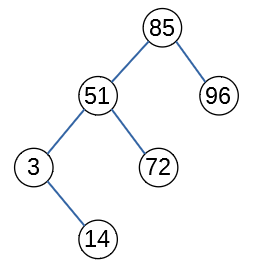
\includegraphics[width=1.5in]{final/splay-tree-initial.png}}
\caption{\label{fig:splay-tree-initial} Intial Tree}
\end{figure}


\vspace{5pt}
{\bf (A)} You have a Binary Search Tree in Figure~\ref{fig:splay-tree-initial}.
Insert two 2-digit numbers: $\overline{ab}$ and also 
$\overline{bc}$ as in a splay tree. (For example, if your Student ID ends with {\tt 789}, 
then the numbers are $78$ and $89$). 

For each insert show the following: 
\begin{itemize}
\item How the tree looks after the insert, but before splaying. 
\item How the tree looks after the splaying (and how many zig-zig, 
zig-zag and/or zig operations you applied). 
\end{itemize}

\vspace{5pt}
{\bf (B)} Could the initial 6-node tree 
appear as a result of six successive node inserts (with splaying upon 
every insert)? 
If so, specify the sequence of six insert commands that would create
the tree in Figure~\ref{fig:splay-tree-initial}.

\newpage



\newpage

\vspace{20pt}
{\bf Question 4 (Graph Algorithm).} 

\begin{figure}[!htb]
\center{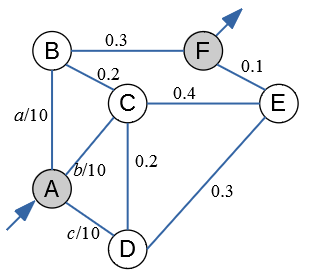
\includegraphics[width=2in]{final/dijkstra-algorithm.png}}
\caption{\label{fig:dijkstra-algorithm} Paths in a Jungle}
\end{figure}

The graph with vertices $A,B,C,D,E,F$ (Figure~\ref{fig:dijkstra-algorithm}) shows 
the available paths in a jungle. Each edge on this 
graph displays the probability that a traveler will 
be bitten by a malaria mosquito and will be infected. 
Assume that mosquito bites are independent
(the event of being bitten on one edge does 
not affect the probability of being bitten on a subsequent edge).
Edges $AB$, $AC$, $AD$ are marked with probabilities $a/10$, 
$b/10$ and $c/10$, where $abc$ is your Student ID number.


\vspace{5pt}
{\bf (A)} Find the {\em best path} from node $A$ to node $F$ such that
the probability to be never bitten is the highest. 

\vspace{5pt}
{\bf (B)} Describe a method (as a pseudocode or 
a precise description) how to compute the best path
in an arbitrary graph $G=(V,E)$ 
(given start and end vertices), 
if the probabilities to be bitten 
are known for every edge. 


\vspace{5pt} 
{\bf (C)} Assume that you 
have Dijkstra's shortest path algorithm (available as a library function): 
It can find the shortest path between any vertices in a weighted undirected graph.  
You also have the graph $G=(V,E)$ for the ``mosquito task'' defined above 
with probabilities $p_{(v,w)} \in [0;1]$ of being 
bitten for every edge $(v,w) \in E$. 

Describe graph and edge weights that you would input into the Dijkstra's algorithm library function
so that it outputs the best path for your ``mosquito task''. (You are allowed to modify 
the input graph itself and also assign any weights you want before passing them into the Dijkstra's algorithm.)


\newpage

{\Large Solutions}

\vspace{10pt}
{\bf Question 1} Assume that Student ID is $\overline{abc} = 789$. 
We need $789+1 = 790$ hash buckets. One hash function (among many possibilities) is the following:

\begin{Verbatim}[frame=single]
/* Possible Solution */
(hash<int>{}(st.birth) ^ 
hash<string>{}(st.string)) % 790
\end{Verbatim}

\vspace{10pt}
{\bf (B)} 

\begin{itemize}
\item {\tt /* EXPR 1 */} This hashfunction is inefficient because of enormous number
of potential collisions: There may be many pairs of students who have 
the birthday weekday (Monday to Sunday) and also the number of characters in their name 
giving the same sum. 
\item {\tt /* EXPR 2 %/} 
\end{itemize}





\end{document}

